\section{Rotary Encoder}
\subsection{Aufgabenstellung}

Auswertung des Drehimpulsgebers

\subsubsection*{Funktionsprototyp}
\begin{itemize}
	\item \texttt{\textcolor{bluetypes}{int8\_t} rotaryEncode()}
\end{itemize}
\subsubsection*{Vorgehensweise}
\begin{enumerate}
	\item Anzeige der Signale mit den auf dem Board vorhandenen LEDs
	\item Entwicklung eines Konzepts zur Auswertung:
	\begin{itemize}
		\item Drehrichtungserkennung
		\item Entprellen?
		\item Kommunikation mit dem aufrufenden Programm		
	\end{itemize}
\end{enumerate}

\subsubsection*{Erweiterte Funktionalität (Schreibmaschine)}
\begin{enumerate}%Aufzählung mit Numerierung
		\item Schreiben und Bearbeiten eines Textes auf dem LC-Display
\end{enumerate}

\subsection{Lösung}
Drehgeber (auch Inkrementaldrehgeber, Quadraturencoder, Drehencoder, Drehimpulsgeber genannt) dienen der dynamischen Erfassung von Winkeländerungen bei Achsen und Wellen. Sie werden sowohl für die manuelle Eingabe von Werten, als auch zur Ermittlung von Drehgeschwindigkeiten eingesetzt.\newline
Inkrementalgeber können mit Schleifkontakten, photoelektrisch, oder magnetisch arbeiten. Sie liefern am Ausgang immer zwei um 90 Grad gegeneinander phasenverschobene Signale (siehe Abbildung \ref{image:Encoder_signal}), anhand deren sich Drehrichtung und -winkel bestimmen lassen. \newline
Die Auswertung des Inkrementalgeber wurde nach dem Zustandsautomat aus Abbildung \ref{image:RotatoryEnode_StateMachine} umgesetzt. Die dazugehörigen Funktionsprototypen sind in Listing \ref{lst:incremental} aufgeführt. \newline
Die Funktion muss zur Initialisierung des Startzustandes zweimal aufgerufen werden, bevor diese aktiv verwendet wird. Weiterhin ist es nötig die Funktion in regelmäßigen Zeitabständen aufzurufen. \newline
\newpage
\begin{figure}[!h]
	\centering
	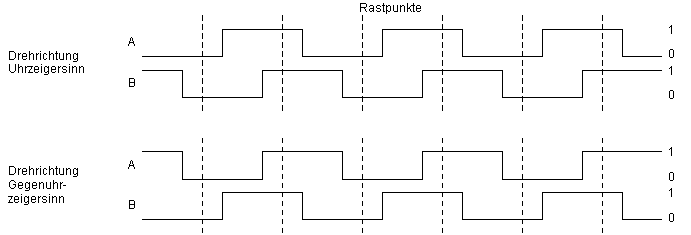
\includegraphics[width=0.85\textwidth]{Images/Encoder_signal}
	\caption[NonBlockingCode]{Signale des Drehimpulsgeber}
	\label{image:Encoder_signal}
\end{figure}

\begin{figure}[!h]
	\centering
	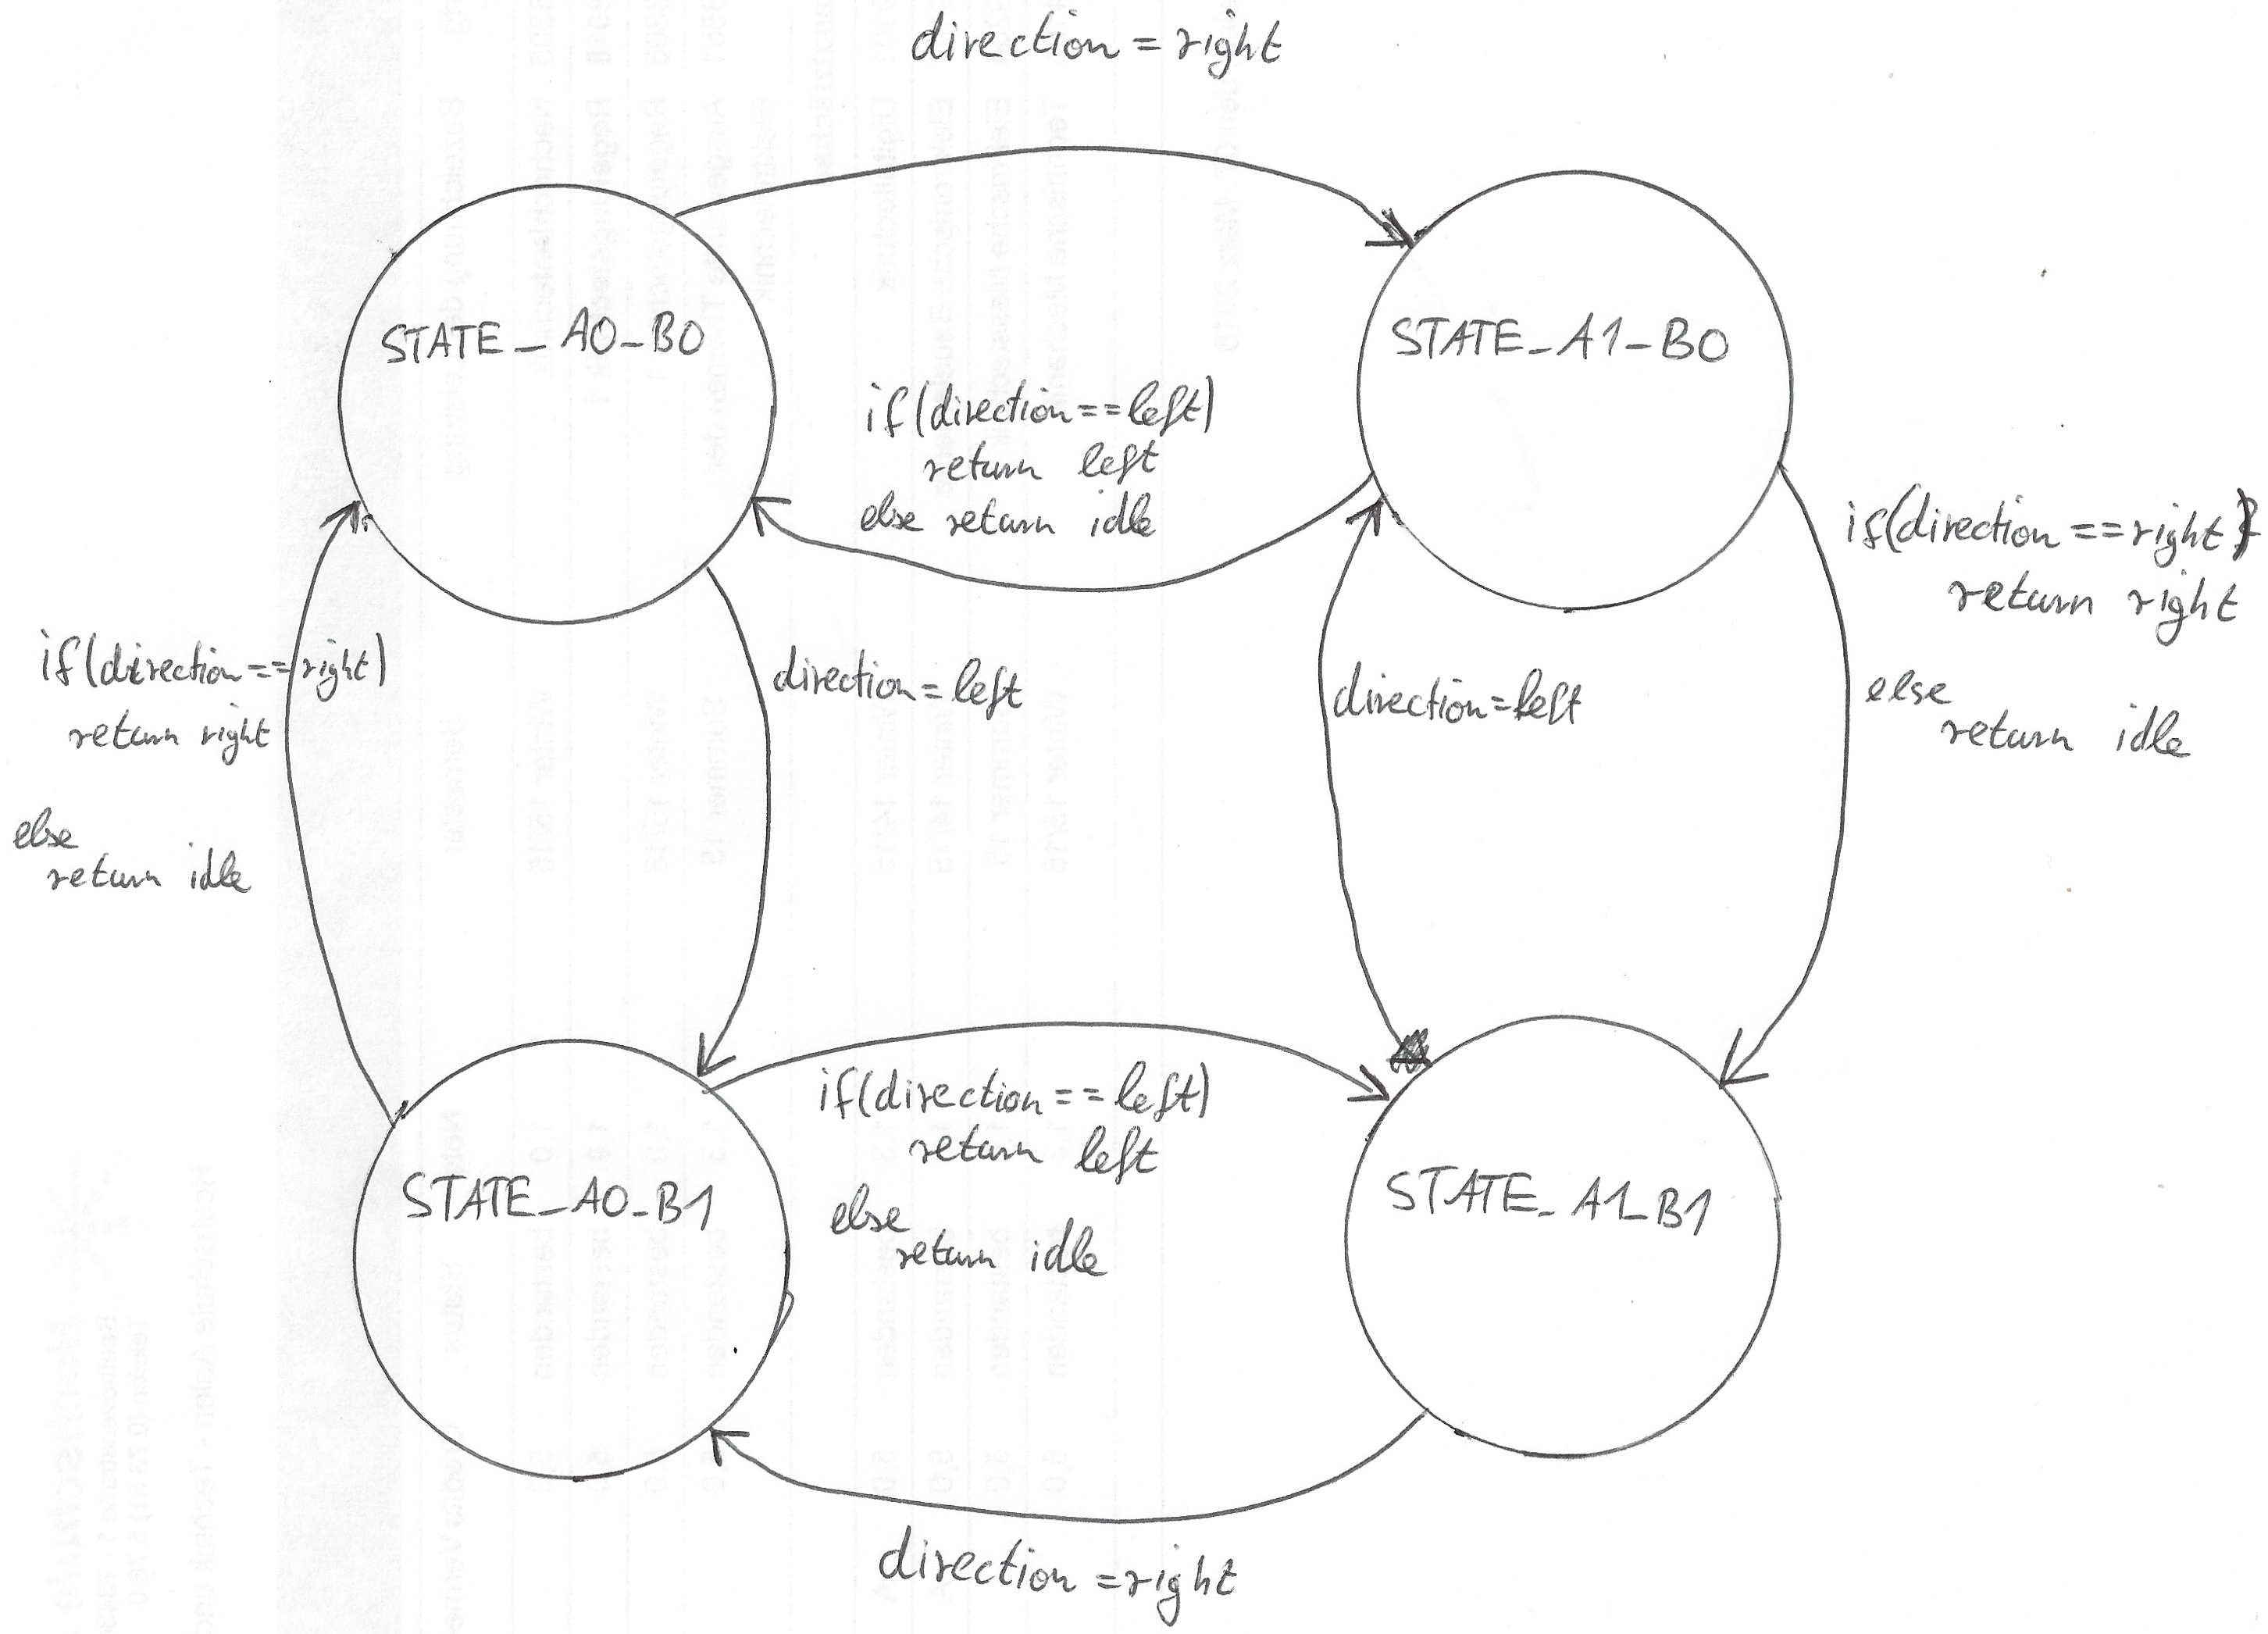
\includegraphics[width=0.85\textwidth]{Images/RotatoryEnode_StateMachine}
	\caption[NonBlockingCode]{Statemachine rotaryEncode()}
	\label{image:RotatoryEnode_StateMachine}
\end{figure}


\begin{lstlisting}[frame=htrbl, caption={Funktionsprototypen für Inkrementalgeber}, label={lst:incremental}]
#define LEFT -1
#define RIGTH 1
#define IDLE 0
#define STATE_A0_B0 0
#define STATE_A1_B0 1
#define STATE_A0_B1 2
#define STATE_A1_B1 3
int8_t rotaryEncode();
\end{lstlisting}

